\documentclass{standalone}
\usepackage{tikz,pgfplots}
\pgfplotsset{compat=newest}

\begin{document}
	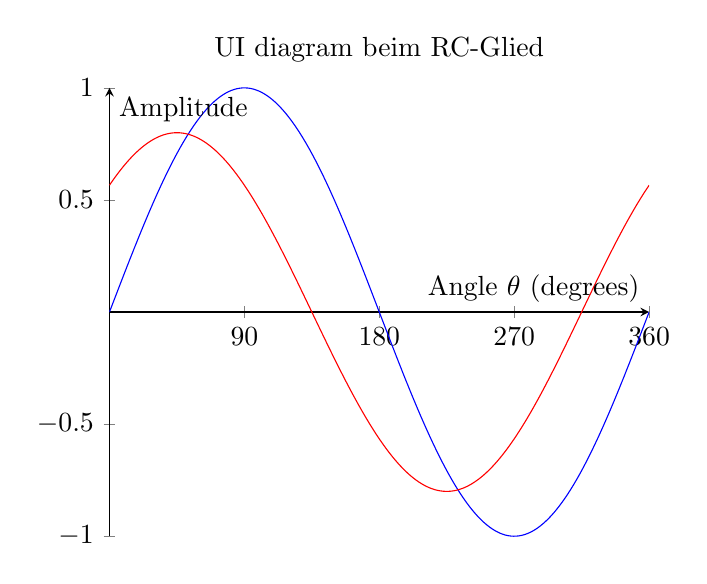
\begin{tikzpicture}
		\begin{axis}[
			title={UI diagram beim RC-Glied},
			domain=0:360,
			samples=200,
			xlabel={Angle $\theta$ (degrees)},
			ylabel={Amplitude},
			xmin=0, xmax=360,
			axis lines = middle,
			xtick={0,90,180,270,360},
			legend pos=north east
		]
		
		% Phase shift (degrees)
		\def\phase{45}
		
		% Voltage
		\addplot[blue]{sin(x)};
		
		% Current
		\addplot[red]{0.8 * sin(x + \phase)};

		\end{axis}	
	\end{tikzpicture}
\end{document}